\section{Approach}
\label{s:approach}
%Approach; What selection of deep uncertainty methods are you using, in what order, and why? This should be clearly motivated and grounded in the literature

% Analysis is carried out across the explicated rival problem framings and relies on state-of- the-art deep uncertainty techniques


%In what order are we using the tools and why are we using them this way
We have opted to combine robust decision making (RDM) and dynamic adaptive policy pathways (DAPP) in our approach to perform risk assessment. DAPP allows for a lot of flexibility, as it represents sequences of promising alternative ways for Gorssel to achieve their objectives as described in Section~\ref{s:prob_frame}. RDM allows us to asses the uncertainty within the variables and analyse their implications. An adaptation tipping point is the point at which a policy does no longer meet the criteria.

We employed TU Delft's open source EMA workbench library which allows for simulations, visualisation and analysis in Python \parencite{kwakkel_exploratory_2017}. An adapted version of the model presented in \citetitle{ciullo_accounting_2019} was used to discover possible strategies. Tool of deltarus to create the metromap.

\begin{longtable}[c]{lp{2cm}p{3cm}l}
\caption{Selected criteria, adaptation objectives, metrics and tolerable impacts}
\label{tab:criteria}\\
\textbf{Criteria}        & \textbf{Adaptation Objective} & \textbf{Metric}                                           & \textbf{Tolerable impact} \\
\hline
\endfirsthead
%
\endhead
%
Land encroachment & TBD & Expected Annual Damage Gorssel & TBD \\
Difference in flood risk & TBD & Difference Expected Number of Deaths Deventer and Gorssel & TBD\\
Difference in protection & TBD & Difference Expected Annual Damage Deventer and Gorssel & TBD
\end{longtable}


\subsection{Generation of scenarios}
Generate the uncertainty space: Generate n number of cases with LHS that incorporate the uncertainties (and store them in a csv file). Alternatively we could use optimisation as well for this.

\subsection{Below for each policy + for base case (without policy) (so iteratively)}
\subsubsection{Identification of adaptation tipping points}
Use scenario discovery (PRIM - so subspace partioning)) to search the results to identify adaptation tipping points. So the results of PRIM are those boxes (which are interesting clusters that contain the interesting cases). (So when we provide PRIM the threshold for outcome, and it will give us the ranges in uncertainty - our triggers).
MOEA might be the most logical to get the Paeto-approximate set of solutions?

\subsubsection{Generation of policies: Directed search to get candidate solutions (policies)}
Generate decision space: GET THEM POLICIES

\subsubsection{Sensitivity analysis}
assess the policies (Sobol, extra trees, Morris)

\subsubsection{Update adaptation pathway}
(so just update it with the new tipping point + policies)


\begin{figure}[h!]
    \centering
    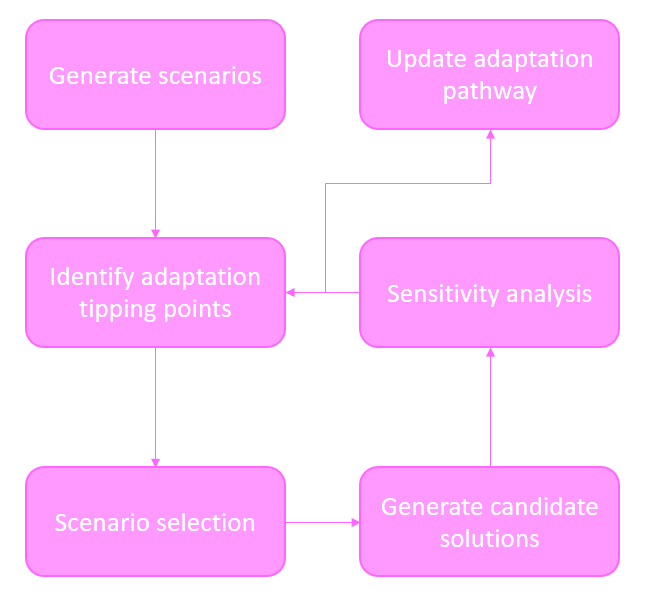
\includegraphics[width=0.25\textwidth]{report/figures/flowchart.png} 
    \caption{Flowchart}
    \label{fig:flowchart}
\end{figure}

\hline




NSGAII-Epsilon - most it can handle is 7-8 objectives. Therefore, the objectives were prioritised.
%Z: to be fair, this is probably also easiest to communicate to the client, lol

Scenario discovery (PRIM)

Directed search(MOEA, MORDM, multi-scenario MORDM, MOE, may need scen disco) $\xrightarrow{}$ sensitivity analysis (Sobol, MOrris, Extra-Trees) $\xrightarrow{}$ Test on found scenarios

%Tools used are unique from policy presentation - you can use MORDM and do policy pathways - CITE: Kwakkel, Haasnoot and Walker, 2015

